\documentclass[a4paper]{article}
\usepackage{xcolor,geometry,palatino}
\addtolength{\parskip}{0.5\baselineskip}
\setlength{\parindent}{0pt}

\usepackage{amsmath}
\usepackage{amssymb}
\usepackage{times}
\usepackage{tikz}

\usetikzlibrary{arrows,automata}

\title{Notes on Probability}
\author{Rich Wareham}

\begin{document}
\maketitle

\section{What is a `probability'?}

Probability is a tricksy beast to define. There are two ways of viewing what
the probability of an event $A$ actually is. These are termed the
\emph{frequentist} and \emph{Bayesian} viewpoints:

\begin{itemize}

\item A frequentist views the probability of an event, $A$ as the ratio between
the number of times that $A$ happened (was true) and the number of times $A$ or
not $A$ happened:
\[
\boxed{ P(A) = \frac{n(A)}{n(A) + n(\lnot A)} }
\]
Notice how we've used $n(A)$ to mean `the number of times $A$ happened' and
$\lnot A$ to mean `not $A$'.

\item A Baysian views the probability of $A$ as measure of our belief that $A$
is true. They use $0$ to show absolute certainty in $\lnot A$ and $1$ to show
absolute certainty in $A$.

\end{itemize}

Either viewpoint can be valid. Should $A$ represent a single result from many
trials, for example tossing a coin and getting a Tail, the frequentist approach
is intuitive and useful. Should $A$ represent a single true/false statement,
for example `this drug is more effective than a placebo', the truth of the
statement does not change each time you ask the question. In such cases
thinking of probability as a measure of belief makes sense. Which view of
probability is useful depends on the problem being addressed.

Also, did you notice the equation up there was boxed? I'll put equations which
are \emph{very} useful definitions and terms to learn in boxes like that.

\section{Random Variables}

Very often one will be asked to find the probability of some \emph{random
variable} having a particular range of values. A random variable is just some
number (or, in general, sets of numbers) we can observe or measure in some
process. For example, a person's height is a random variable: until we measure
it, we cannot say with certainty what it is.

Usually a random variable is denoted with a capital letter and a particular
observation of that random variable with a lower-case letter. For example we
may use $H$ to mean `the height of a person' and $h$ to mean `the measured
height of a particular person'.

For example we can read $P(H \le 180\mbox{cm})$ as `the probability that the
height of a person is less than or equal to 180cm'. Similarly we can read $P(H
\le h)$ as `the probability that the height of a person is less than or equal
to $h$'. Notice how $H$ always stands for `the height of a person' whereas $h$
stands for a particular height (e.g. 180cm or 137.5cm).

What this means in practise is that if you have a function which deals with
probability, all the arguments to that function which are numbers should be
lower-case!

Often this can be confusing so below, when we present some common functions,
we'll use $\blacklozenge$ to mean `a random variable' (e.g.\ $H$) and
$\lozenge$ to mean `the value of a random variable' (e.g.\ $h$). When using the
definitions of these functions you can substitute the $\blacklozenge$ and
$\lozenge$ appropriately.

Remember: $\blacklozenge$ is just a label which tells us what random variable
we're dealing with, $\lozenge$ is that variable's actual value.

\section{The Cumulative Distribution Function}

The Cumulative Distribution Function (CDF) is, in essence, the starting point
from which everything else you'll use in probability derives. It is simply a
function that tells us something about the value of a random variable. In fact
it tells us the probability that a random variable will have a particular value
or lower. The CDF for the random variable $\blacklozenge$ is defined to be: 
\[
\boxed{ F_\blacklozenge(\lozenge) = P(\blacklozenge \le \lozenge) }
\]

Recall that $\blacklozenge$ is just a label telling us what the random variable
is. We could write down the definition of the CDF for the height of a person by
simply substituting $H$ and $h$:
\[
F_H(h) = P(H \le h).
\]

\subsection{Free variables}

Now, it is only a convention that we use corresponding lower-case letters to
denote particular values of the random variable. The CDF for the height of a
person could just as easily been written as $F_H(x) = P(H \le x)$. The
important thing is that we know what random variable we're talking about.
Variables, like $h$, which we are free to re-name---assuming we do it
consistently---are called \emph{free variables}.

It is important to note what variables are free variables since it is often the
case that a proof can be completed by just changing an $x$ to a $y$ in the
right place!

\subsection{Why not just talk about $P(\blacklozenge = \lozenge)$?}

So why do we use $P(\blacklozenge \le \lozenge)$ instead of $P(\blacklozenge =
\lozenge)$? Well, the answer is surprising: for many random variables the value of
$P(\blacklozenge = \lozenge)$ is always zero!

Imagine, for a moment, that $\blacklozenge$ is `the hour shown on a clock'
which we'll call $C$. If we assume this is a usual 12-hour clock, there are 12
distinct values that $C$ can take. Let's use the frequentist approach to
calculate $P(C = c)$:

\begin{itemize}

\item If we look at the clock $N$ times at random we'd expect on average one
twelfth of the time to find that the hour is $c$ so $n(C = c) = N/12$ if $1 \le
c \le 12$ and zero otherwise.

\item The rest of the time $C \ne c$ and so $n(C \ne c) = 11N / 12$ if $1 \le c
\le 12$ and $n(C \ne c) = N$ otherwise.

\item Using the frequentist definition of probability, therefore,
\[
P(C = c) = \left\{
\begin{array}{c l l}
\frac{N/12}{N/12 + 11N/12} & = 1/12 & \mbox{if } 1 \le c \le 12 \\
0 / N & = 0 & \mbox{otherwise}
\end{array}
\right.
\]

\end{itemize}

All fine and good. But now consider $\blacklozenge$ being `the angle the hour
hand makes with the vertical', or $A$. Again consider the frequentist approach.

\begin{itemize}

\item There is one and only one case when $A = a$ so $n(A = a) = 1$.

\item There are an infinity of angles which are not $a$ so $n(A \ne a) = \infty$.

\item Hence $P(A = a) = 1 / \infty = 0$.

\end{itemize}

The argument above justifies our assertion that some random variables end up
with the probability of them taking any one value as being zero. To restate:
there are an infinity of possible angles that the hour hand can take so,
assuming them all to be equally likely, the probability of any one of them is
zero.

For most random variables it often makes more sense to consider the probability
of them taking a \emph{range} of values. For example, if the hour hand has
angle $a$ corresponding to hour $c$ then it follows that $(c-1) \times 30^\circ
< a \le c \times 30^\circ$. It should be possible to convince yourself it
follows that
\[
P(C = c) = P(A \le c \times 30^\circ) - P(A \le (c-1) \times 30^\circ),
\]
or, making use of the CDF for $A$:
\[
P(C = c) = F_A(c \times 30^\circ) - F_A((c-1) \times 30^\circ).
\]

Notice that the CDF for $A$ is actually useful and has a sensible value. If
every position of the hour hand is equally likely then $F_A(0^\circ) = 0$ and
$F_A(360^\circ) = 1$. If we were to plot the value of $F_A$ it would look
something like this:

{\center
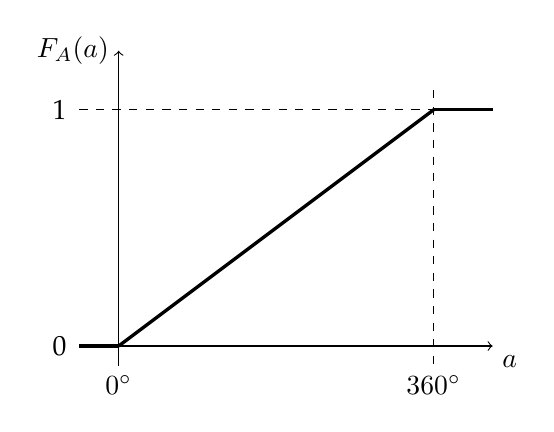
\begin{tikzpicture}
% axes
\draw[->] (-.5,0)--(4.75,0) node[below right]{$a$};
\draw[->] (0,-.25)--(0,3.75) node[left]{$F_A(a)$};

% the CDF
\begin{scope}[very thick]
\draw (-.5,0)--(0,0);
\draw (0,0)--(4,3);
\draw (4,3)--(4.75,3);
\end{scope}

% the bounds
\begin{scope}[dashed]
\draw (-.5,3)--(4.25,3);
\draw (4,3.25)--(4,-.25);
\end{scope}

% y-axis
\draw (-.75,3) node{1};
\draw (-.75,0) node{0};

% x-axis
\draw (4,-.5) node{$360^\circ$};
\draw (0,-.5) node{$0^\circ$};
\end{tikzpicture} \\ \null
}
We can even write down an explicit equation for $F_A$:
\[
F_A(a) = \left\{
\begin{array}{cl}
a / 360^\circ & \mbox{if } 0^\circ \le a < 360^\circ \\
0 & \mbox{otherwise.}
\end{array}
\right.
\]

It is instructive to use this definition of $F_A(a)$ to convince yourself
that it can be used to show that $P(C=c) = 1/12$ for valid $c$.

\subsection{The Gaussian CDF}

There is a CDF which often comes up when measuring `natural' random variables
(like the height of a person) called the \emph{Gaussian} CDF. You may also have
heard it called the \emph{normal distribution}. Let's not worry for the moment
exactly how hit is defined, instead lets just take a look at it:

{\center
\fbox{
\begin{tikzpicture}
% axes
\draw[->] (-.5,0)--(4.75,0) node[below right]{$g$};
\draw[->] (2,-.25)--(2,3.75) node[left]{$F_G(g)$};

% the CDF
\begin{scope}[very thick]
\draw plot[id=gaussian-cdf,domain={-.5:4.75}] function{3*0.5*(1+erf((x-2)/((2.0/3.0)*sqrt(2))))};
\end{scope}

% the bounds
\begin{scope}[dashed]
\draw (-.5,3)--(4.25,3);
\draw (-.5,1.5)--(4.25,1.5);
\draw (4,3.25)--(4,-.25);
\draw (0,3.25)--(0,-.25);

\draw (-.5,0.5)--(4.25,0.5);
\draw (-.5,2.5)--(4.25,2.5);
\draw (1.333,3.25)--(1.333,-.25);
\draw (2.666,3.25)--(2.666,-.25);
\end{scope}

% y-axis
\draw (-.5,3) node[left]{1};
\draw (-.5,1.5) node[left]{0.5};
\draw (-.5,0) node[left]{0};

\draw (-.5,0.5) node[left]{$\frac{1}{6}$};
\draw (-.5,2.5) node[left]{$\frac{5}{6}$};

% x-axis2
\draw (0,-.5) node{$-3$};
\draw (1.333,-.5) node{$-1$};
\draw (2,-.5) node{$0$};
\draw (2.666,-.5) node{$1$};
\draw (4,-.5) node{$3$};
\end{tikzpicture}} \\ \null
}

Notice that this is in a box. Being able to sketch the Gaussian CDF is
\emph{very} useful. We can already see some things from this picture. For
instance, there is a 0.5 probability of $G \le 0$. Also there is a probability
of approximately $2/3$ that values are within $\pm 1$ of zero\footnote{The
actual probability is more like 0.682.}. The Gaussian is well suited to random
variables whose values cluster around some central point and are spread equally
either side.

We find the Gaussian is often a good fit for `natural' random variables like
the height of a person. Here is the CDF of measured heights for women in the
U.K.

{\center
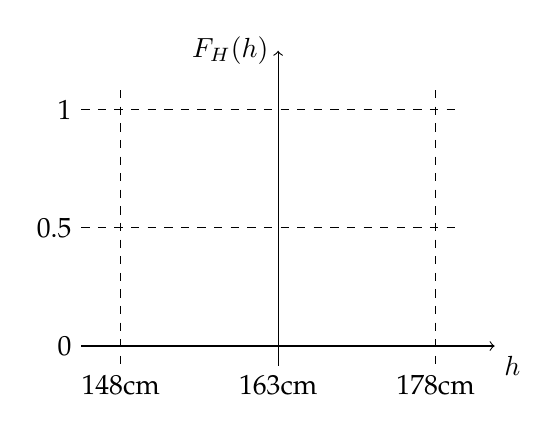
\begin{tikzpicture}
% axes
\draw[->] (-.5,0)--(4.75,0) node[below right]{$h$};
\draw[->] (2,-.25)--(2,3.75) node[left]{$F_H(h)$};

% the CDF
\begin{scope}[very thick]
\draw plot[id=gaussian-cdf,domain={-.5:4.75}] function{3*0.5*(1+erf((x-2)/((2.0/3.0)*sqrt(2))))};
\end{scope}

% the bounds
\begin{scope}[dashed]
\draw (-.5,3)--(4.25,3);
\draw (-.5,1.5)--(4.25,1.5);
\draw (4,3.25)--(4,-.25);
\draw (0,3.25)--(0,-.25);

%\draw (-.5,0.5)--(4.25,0.5);
%\draw (-.5,2.5)--(4.25,2.5);
%\draw (1.333,3.25)--(1.333,-.25);
%\draw (2.666,3.25)--(2.666,-.25);
\end{scope}

% y-axis
\draw (-.5,3) node[left]{1};
\draw (-.5,1.5) node[left]{0.5};
\draw (-.5,0) node[left]{0};

%\draw (-.5,0.5) node[left]{$\frac{1}{6}$};
%\draw (-.5,2.5) node[left]{$\frac{5}{6}$};

% x-axis2
\draw (0,-.5) node{148cm};
%\draw (1.333,-.5) node{158cm};
\draw (2,-.5) node{163cm};
%\draw (2.666,-.5) node{168cm};
\draw (4,-.5) node{178cm};
\end{tikzpicture} \\ \null
}

Notice that it's pretty much the same shape as the Gaussian. In fact we can
stretch and scale the Gaussian CDF to fit the data:
\[
F_H(h) = F_G\left( \frac{h - 163\mbox{cm}}{5\mbox{cm}} \right).
\]

We can generalise this stretching and scaling to fit a Gaussian random variable
centred on $\mu$ and with around 2/3 of the observed values within $\sigma$ of
$\mu$. Let's call this random variable $X_g$. We can write down the CDF for
$X_g$ in terms of a stretched version of $F_G$:
\[
\boxed{ F_{X_g}(x;\mu,\sigma) = F_G\left( \frac{x - \mu}{\sigma} \right) }
\]
We term $\mu$ the \emph{mean} and $\sigma$ the \emph{standard deviation}. We'll
return to these later and define them properly but for now just think of them
as knobs to control the shape of the Gaussian CDF. The random variable $G'$ is
still Gaussian, it's just been stretched and scaled. We differentiate a
Gaussian random variable with $\mu = 0$ and $\sigma = 1$ (i.e.\ $G$) by calling
it the \emph{standard} Gaussian.

We call these knobs \emph{parameters} and we differentiate them from random
variable values by putting them after a `;' in the function arguments.

\section{The Probability Density Function}

\[
\boxed{ 
f_\blacklozenge(\lozenge) = \frac{d}{d \lozenge} F_\blacklozenge(\lozenge) 
\quad \Leftrightarrow \quad
F_\blacklozenge(\lozenge) = \int_{-\infty}^\lozenge f_\blacklozenge(\heartsuit) \, \mbox{d}\heartsuit
}
\]

\fbox{\parbox{0.9\textwidth}{
{
\[
F_\blacklozenge(\lozenge) \triangleq P(\blacklozenge \le \lozenge)
\]
\center
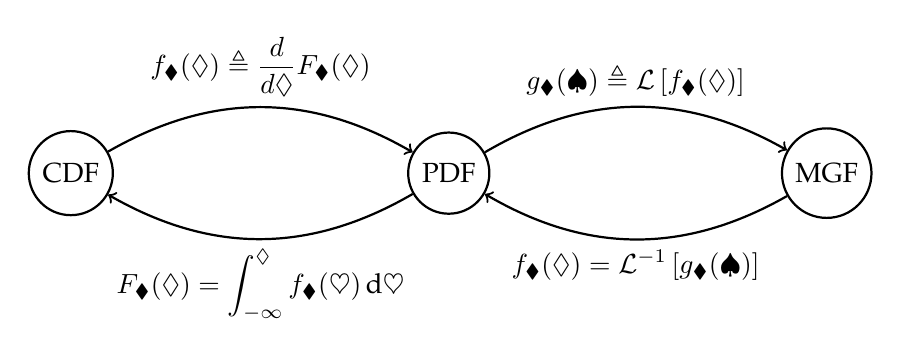
\begin{tikzpicture}[->,node distance=4.8cm,thick]
%\tikzstyle{every state}=[fill=red,draw=none]
\node[state] (PDF) {PDF};
\node[state] (CDF) [left of=PDF] {CDF};
\node[state] (MGF) [right of=PDF] {MGF};

\path (PDF) edge [bend left,below] node {$\displaystyle F_\blacklozenge(\lozenge) = \int_{-\infty}^\lozenge f_\blacklozenge(\heartsuit) \, \mbox{d} \heartsuit$} (CDF)
            edge [bend left,above] node {$\displaystyle g_\blacklozenge(\spadesuit) \triangleq \mathcal{L}\left[f_\blacklozenge(\lozenge)\right]$}(MGF);
\path (CDF) edge [bend left,above] node {$\displaystyle f_\blacklozenge(\lozenge) \triangleq \frac{d}{d\lozenge} F_\blacklozenge(\lozenge)$} (PDF);
\path (MGF) edge [bend left,below] node {$\displaystyle f_\blacklozenge(\lozenge) = \mathcal{L}^{-1}\left[ g_\blacklozenge(\spadesuit) \right]$} (PDF);
\end{tikzpicture} \\ \null 
{\footnotesize $\heartsuit$ and $\spadesuit$ are \emph{free variables};
$\blacklozenge$ is the \emph{name} of a random variable;
$\lozenge$ is a particular \emph{value} of $\blacklozenge$.\\} 
}}}

\end{document}

% vim:sw=4:ts=4:et:spell:spelllang=en_gb
